\section{Summary of Paper \ref{pap:pit}}
\subsection*{"\nameref{pap:pit}"}
\subsection*{Scope and motivations}
In order to expand the modeling complexity and uncertainty from Paper \ref{pap:rolldamping}, system identification of manoeuvring by adding the the surge, sway, and yaw degrees of freedom was studied in Paper \ref{pap:pit}. 
The objective was to find parametric model structures with good generalization and to develop parameter identification techniques from FRMT data.

The dynamics were assumed to be described by an Abkowitz or truncated Abkowitz model. 
The system identification method proposed in Paper \ref{pap:pit} was validated on two case study ships: the wPCC and the KVLCC2 (\autoref{fig:kvlcc2_hsva}). The parameters were identified with recursive inverse dynamics regression (see \autoref{sec:RIDR}).
The identification was carried out with cross validation using hold-out evaluation \cite{sammutHoldoutEvaluation2017}.
The data in this evaluation were divided into three sets: the training set, the validation set and the test set as seen in \autoref{fig:model_development_process}.
The purpose of the training set was to train all the candidate models using the proposed parameter estimation method. The validation set was used to select the most effective candidate model. The training and validation sets were joined to train the selected model as the final model. The final model was used for predicting the test set, which was used to evaluate the accuracy of the model. These three sets were not divided randomly;  they were divided to assess the model’s extrapolation ability. The data sets were therefore split to have the smallest yaw rates, drift-angles, and rudder-angles in the training set; the medium values in the validation set; and the largest values in the test set.
Examples of this can be seen for the two test cases in \autoref{fig:wpcc_datasets} and \autoref{fig:kvlcc2_datasets}.
%\begin{figure}[h!]
%\centering
%\includegraphics[width=0.5\linewidth]{kappa/images/wpcc_mdl.png}
%\caption{wPCC tested at SSPA Maritime center. Copyright 2020 by RISE.}
%\label{fig:wpcc-mdl}
%\end{figure}
\begin{figure}[h!]
    \centering
    \begin{subfigure}[b]{0.45\textwidth}
    \centering
    \includegraphics[height=3cm]{kappa/images/kvlcc2_front.png}
    \end{subfigure}
    ~
     \begin{subfigure}[b]{0.45\textwidth}
     \centering
     \includegraphics[height=3cm]{kappa/images/kvlcc2_aft.png}
     \end{subfigure}
+    \caption{Ship model used in HSVA and MARIN model tests. Copyright HSVA.}
    \label{fig:kvlcc2_hsva}
\end{figure}
\begin{figure}[H]
\centering
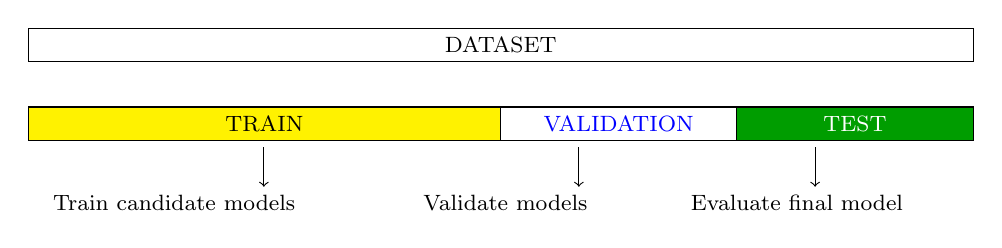
\begin{tikzpicture}

\node (dataset)[rectangle,
    anchor=west,
    draw,
    text = black,
    minimum width=12cm,
    fill = white] at (0, 0) {\footnotesize DATASET};

\node (train)[rectangle,
    draw,
    anchor=west,
    text = black,
    minimum width=6cm,
    fill = yellow] at (0, -1cm) {\footnotesize TRAIN};

\node (validation)[rectangle,
    draw,
    anchor=west,
    text = blue,
    minimum width=3cm,
    fill = white] at (6cm, -1cm) {\footnotesize VALIDATION};

\node (test)[rectangle,
    draw,
    anchor=west,
    text = white,
    minimum width=3cm,
    fill = black!15!green!255] at (9cm, -1cm){\footnotesize TEST};
    
\node (train_multiple)[rectangle,
    draw,
    anchor=west,
    text = black,
    draw = none,
    fill = none] at (0.2cm, -2cm){\footnotesize Train candidate models};
    
\node (validate_models)[rectangle,
    draw,
    anchor=west,
    text = black,
    draw = none,
    fill = none] at (4.9cm, -2cm){\footnotesize Validate models};
    
\node (evaluate_models)[rectangle,
    draw,
    anchor=west,
    text = black,
    draw = none,
    fill = none] at (8.3cm, -2cm) {\footnotesize Evaluate final model};

\draw[->] (3,-1.3) -- (3,-1.8);
\draw[->] (7,-1.3) -- (7,-1.8);
\draw[->] (10,-1.3) -- (10,-1.8);
\end{tikzpicture}
\caption{Model development process with hold-out evaluation.}
\label{fig:model_development_process}
\end{figure}
\begin{figure}[h!]
\centering
\includegraphics[width= 1.0\linewidth]{kappa/images/3.pdf}
\caption{wPCC training, validation and testing datasets.}
\label{fig:wpcc_datasets}
\end{figure}
\begin{figure}[h!]
\centering
\includegraphics[width=1.0\textwidth]{kappa/images/4.pdf}
\caption{KVLCC2 training, validation and testing datasets.}\label{fig:kvlcc2_datasets}
\end{figure}

\subsection*{Results and concluding remarks}
\autoref{fig:validation-forces} shows predictions of the wPCC validation set with the identified models. AVMM is a full Abkowitz model and MAVMM is a truncated Abkowitz model where model structure selection has been applied. The AVMM model over-predicted the forces by far. 
This over-prediction was  explained by the high multicollinearity of the AVMM model structure for the wPCC data as shown in \autoref{fig:ncorr}  where the absolute correlation coefficient between the features in the wPCC yaw moment regression is presented.
Therefore, simulations of the validation cases were only possible using the MAVMM. 
The MAVMM model was retrained on the joined test and validation data set to obtain the final prediction model which was used to predict the turning circle test data set as shown in \autoref{fig:track-plot-testing-sim}. Advance and tactical diameter \cite{imoStandardsShipManoeuvrability2002} from the prediction differs by 4\% and 1\%. Monte Carlo simulations with alternative realizations of the regression, considering the uncertainty in the regressed parameters, are also displayed in these figures. The alternative realizations have similar simulation results to the model with mean values of the regression (black line).
\begin{figure}[h]
\centering
\includegraphics[width=1.0\textwidth]{kappa/images/7.pdf}
\caption{Validation of force models for wPCC ZigZag20/20.}\label{fig:validation-forces}
\end{figure}
\begin{figure}[h]
\centering
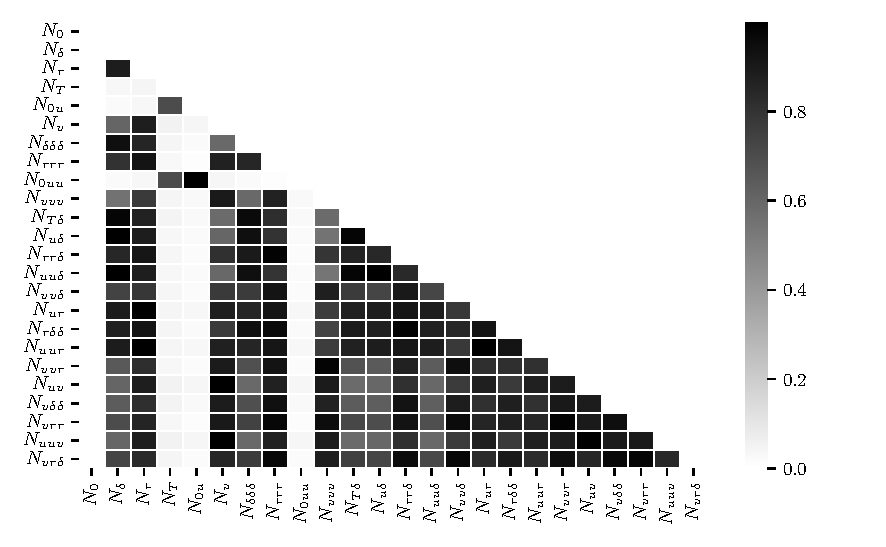
\includegraphics[width=1.0\textwidth]{kappa/images/10.pdf}
\caption{Absolute correlation between the features in the wPCC yaw moment regression of AVMM.}\label{fig:ncorr}
\end{figure}
\begin{figure}[h]
    \centering

    \begin{subfigure}[b]{\textwidth}
        \includegraphics[width=0.90\textwidth]{kappa/images/11.pdf}
        \caption{Track plots.}\label{fig:track-plot-testing-sim}
    \end{subfigure}
    \vfill
    \begin{subfigure}[b]{\textwidth}
        \includegraphics[width=0.90\textwidth]{kappa/images/12.pdf}
        \caption{Time series.}\label{\detokenize{06.10_results_wpcc:fig-testing-sim}}
    \end{subfigure}
        
    \caption{Turning circle test case for wPCC from model test and simulations.}
    \label{fig:enter-label}
\end{figure}

%\includegraphics[width=0.90\textwidth]{kappa/images/11.pdf}
%\caption{Turning circle test case for wPCC, track plots from model test and simulation.}\label{fig:track-plot-testing-sim}
%\end{figure}
%\begin{figure}[ht]
%\centering
%\includegraphics[width=0.90\textwidth]{kappa/images/12.pdf}
%\caption{Turning circle test case for wPCC, time series from model test and simulation.}\label{\detokenize{06.10_results_wpcc:fig-testing-sim}}\end{figure}
\FloatBarrier

The corresponding final prediction of the turning circle test for the KVLCC2 test case is shown in \autoref{fig:fig-kvlcc2-track-plot-testing-sim}. The prediction was conducted using simulation with the MAVMM trained on the training and validation datasets. Monte Carlo simulations with alternative realizations of the regression are also displayed in this figure. The alternative realizations are very similar to the model with mean values of the regression (black line).
The predicted advance and tactical diameters differ by 2\% and 5\%.
\begin{figure}[h]
    \centering

    \begin{subfigure}[b]{0.80\textwidth}
        \includegraphics[width=\textwidth]{kappa/images/17.pdf}
        \caption{Track plots.}
    \end{subfigure}
    \vfill
    \begin{subfigure}[b]{0.80\textwidth}
        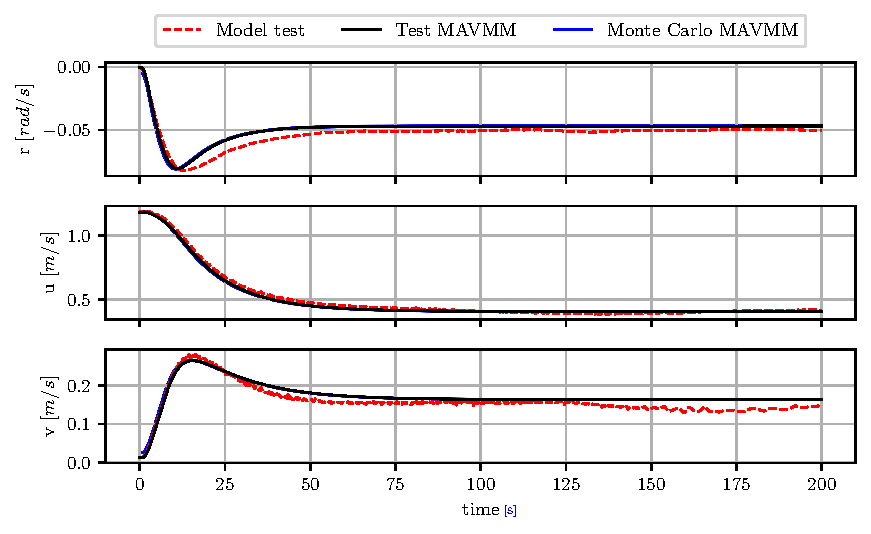
\includegraphics[width=\textwidth]{kappa/images/18.pdf}
        \caption{Time series}
    \end{subfigure}
        
    \caption{Comparison between the predicted turning circle test with MAVMM trained on HSVA data and MARIN model test results for KVLCC2.}
    \label{fig:fig-kvlcc2-track-plot-testing-sim}
\end{figure}
\clearpage